\subsection{Ladestation} \label{sec:ladestation}

Nachdem die gesamte induktive Ladeschaltung und Energiespeicherung beschrieben wurde, folgt nun die Beschreibung der Ladestation. Hierfür wurde ein Prototyp erstellt, welcher die gesamte primäre induktive Ladeschaltung beinhaltet. Für den Prototypen wurde eine .stl Datei erstellt, welche mit einem 3D-Drucker gedruckt wurde. Wichtig ist hierbei zu erwähnen, dass es sich nur um einen Prototypen handelt und es bei einer Weiterentwicklung noch Anpassungen geben kann. Da die Ladestation für Versuchszwecke erstellt wurde, ist das Design so gewählt, dass nur ein Dōjō geladen werden kann. Dies könnte in einem weiteren Schritt auf mehrere Ladeaussparungen erweitert werden, wodurch mehrere Dōjōs gleichzeitig pro Ladestation geladen werden können. Abbildung \ref{fig:Prototyp} zeigt die Ladestation aus verschiedenen Perspektiven.

\begin{figure}[htbp]
	\centering
	\subfigure[Frontansicht]{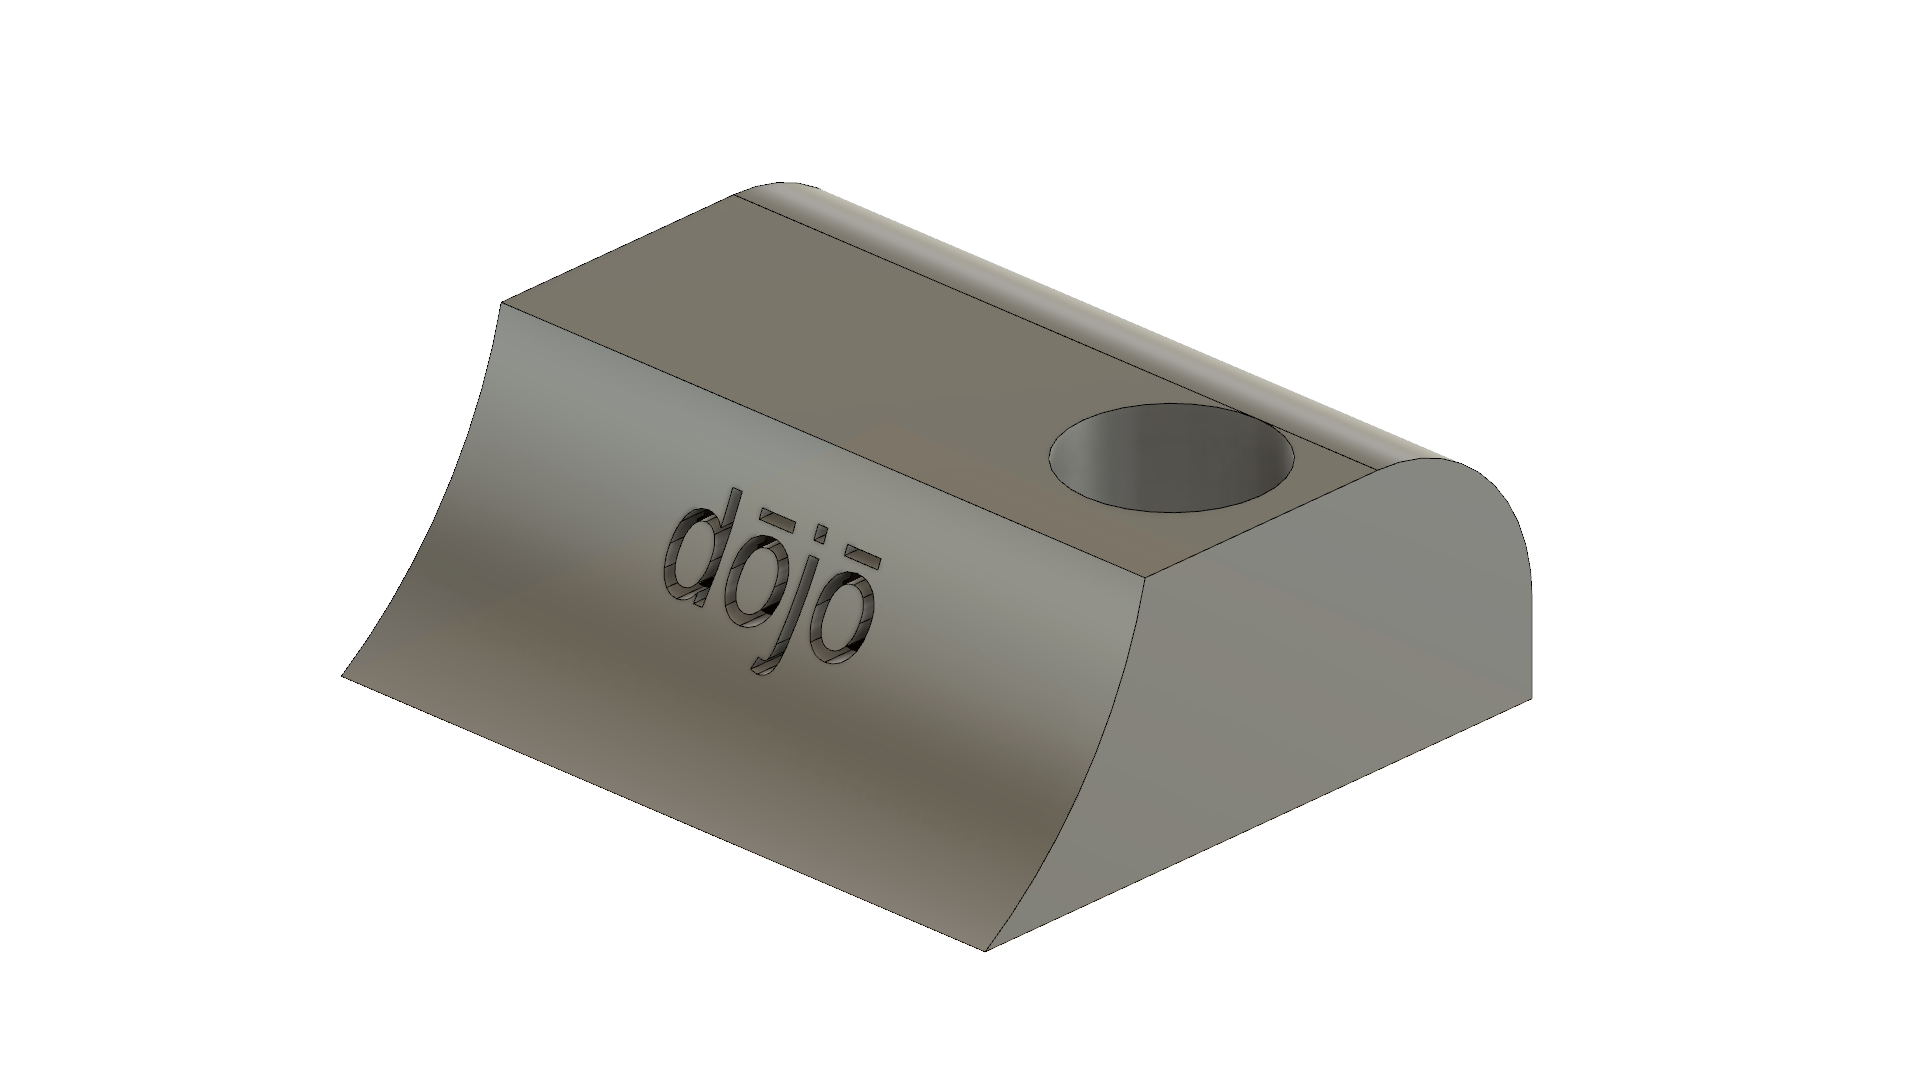
\includegraphics[width = 0.3\textwidth]{data/DojoLadestation01.png}}\quad
	\subfigure[Sicht von oben]{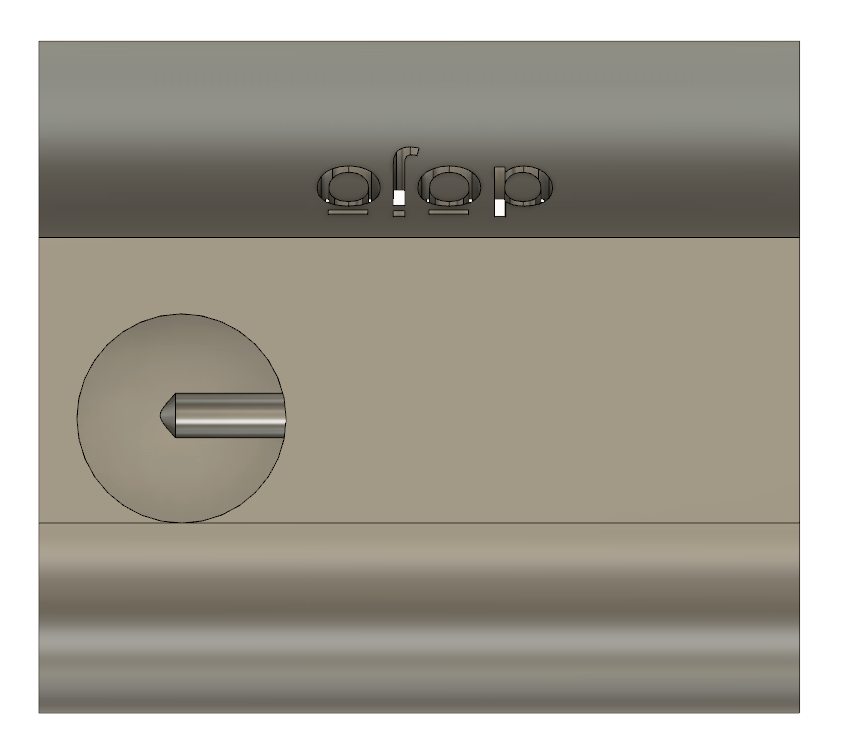
\includegraphics[width = 0.3\textwidth]{data/DojoLadestation02.png}}\quad
	\subfigure[Sicht von unten]{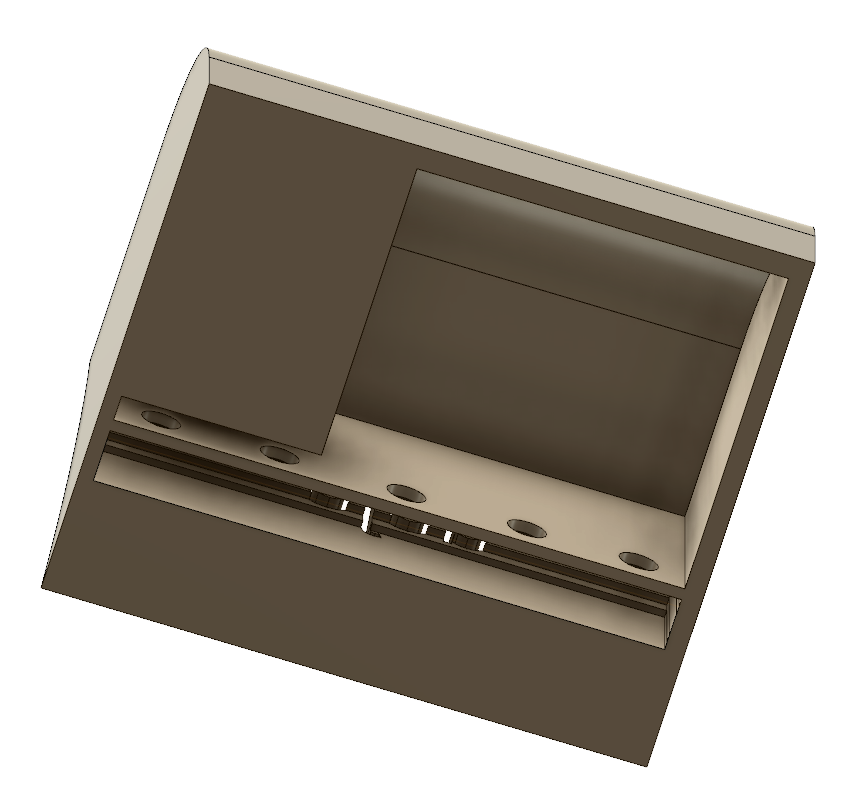
\includegraphics[width = 0.3\textwidth]{data/DojoLadestation03.png}}
	\caption[Prototyp Ladestation]{Prototyp der Ladestation aus verschiedenen Perspektiven}
	\label{fig:Prototyp}
\end{figure}

Die Öffnung dient zum einen als Standhalterung und zum anderen als korrekte Positionierung für die induktive Ladeschaltung. Die richtige Positionierung ist eines der wichtigsten Kriterien für einen optimalen Ladezyklus, da die Transceiver- und Receiverspule direkt übereinanderliegend den besten Wirkungsgrad erzielen. Der Hohlraum im Inneren der Ladestation dient zur Platzierung des Primärkreises und hat die Abmessung (80 x 70.7 x 30)mm. Für den Prototypen wurde eine Lochrasterplatine mit allen nötigen Komponenten gefertigt, welche genau in diese Aussparung passt. Weiter sind runde Löcher (5mm $\o$) ersichtlich, welche in die Kammer des Schriftzuges führen. Sie sind für LEDs vorgesehen, welche den Dōjō-Schriftzug bei angeschlossener Versorgungsspannung zum Leuchten bringen.